


\subsection{WP 1.2 — Gestion des échanges données et du microcontrôleur (responsable : Nolan Buchet)}

\subsubsection{Rappel des objectifs}

Pour recontextuatlisé le projet et les objectifs de ce Work Package, le WP 1.2 fait partie du Work parckage 1 qui 
est dédié à la conception et au développement du système de collecte de données animalières. Le WP 1.2 se concentre 
spécifiquement sur la gestion des échanges de données entre les différents composants du système, ainsi que sur 
l'intégration et la programmation du microcontrôleur qui servira de cerveau central pour le projet. De plus celui-ci 
s'occupera de la partie énergétique du module, ainsi que de la partie stockage des données collectées.
\\

Voici la liste des taches qui seront réalisées dans le cadre de ce WP :
\begin{itemize}
    \item Tache 0 ( Equipe ) : Choix du Microcontrôleur et de la carte SD
    \item Tache 1 : Gestion du stockage des données collectées
    \item Tache 2 ( hors WP ) : Gestion de la luminosité pour WP 1.3
    \item Tache 3 ; Gestion de l'horodatage et de la localisation du modules
    \item Tache 4 : Définition d'un Automate pour la gestion global du module
    \item Tache 5 : Développement d'une architecture electrique
    \item Tache 6 : Intégration des modules ( prototypage )
    \item Tache 7 : Gestion de l'alimentation du module
    \item Tache 8 : Création d'un PCB pour le module
    \\
\end{itemize}

Pour chacune des taches réalisée ci-dessus, il y a eu une phase de test réalisé, ainsi qu'en amont une phase de concertation avec 
l'équipe du WP afin que les solutions envisagées soient en adéquation avec les besoins du projet.
\\

Certaines tâches de ce modules ne sont pas dans l'ordre de conception, en prenant la tache 4 ou 5 qui ont été en constante évolution 
durant tout le projet. Et certaine taches non essentielle, mais logique, comme l'optimisation des codes, ou rapport / documention ont 
été réalisé en parallèle de la conception du module.
\\

\subsubsection{Tache 0 : Choix du Microcontrôleur}

\subsubsection*{Solution envisagé}

À la suite d’une phase de recherche ( benchmark du début de projet ) concernant le contrôleur à utiliser pour ce projet, nous avons identifié deux solutions susceptibles 
de répondre à nos besoins : l’ESP32 et le Raspberry Pi Zero.
\\

Pour rappel, les besoins principaux concernant le contrôleur étaient les suivants :
\\

\begin{center}
\renewcommand{\arraystretch}{1.3}
\begin{tabularx}{0.9\textwidth}{>{\bfseries}l|X}
\toprule
\textbf{Critère} & \textbf{Description} \\
\midrule
Consommation énergétique & Minimiser la consommation pour un usage sur batterie. \\ 
Performances & Garantir une puissance suffisante pour le traitement des données. \\ 
Stockage & Disposer d’une capacité suffisante pour enregistrer temporairement les mesures locales et la photographie. \\ 
Système & Offrir un environnement logiciel simple avec facilité sur les outils de développement utilisés. \\ 
Interfaces & Proposer des entrées/sorties adaptées aux capteurs et modules externes. \\ 
Connectivités & Intégrer ou supporter le Wi-Fi, le Bluetooth ou d'autres moyens de communication. \\ 
Prix & Rester dans une gamme de coût compatible avec le budget du projet. \\ 
\bottomrule
\end{tabularx}
\end{center}

Ces critères nous ont permis de comparer plusieurs solutions techniques lors de la phase de benchmark.
\\

Les critères suivants ont été considérés lors du choix final du microcontrôleur :
\begin{itemize}
    \item Architecture matérielle
    \item Connectivité
    \item Consommation énergétique
    \item Nombre et type de GPIO
    \item Facilité de développement
    \item Coût global
    \\
\end{itemize}

À l’issue de l’analyse comparative réalisée entre l’ESP32 et le Raspberry Pi Zero, le choix s’est porté sur l’ESP32 comme microcontrôleur 
principal pour le collecteur de données animalières. Ce choix est motivé par plusieurs facteurs clés. Tout d’abord, sa faible consommation
énergétique constitue un avantage décisif pour une utilisation sur batterie dans un environnement isolé. L’ESP32 peut fonctionner 
plusieurs jours, voire semaines, en mode basse consommation, ce qui garantit une autonomie optimale sur le terrain.
\\

Ensuite, son intégration native du Wi-Fi et du Bluetooth simplifie la conception matérielle et réduit le besoin de modules externes, 
tout en permettant la transmission sans fil des données et la configuration à distance du système.
\\

Enfin, son coût réduit et sa disponibilité sur le marché en font une solution économique et accessible, sans compromis majeur sur 
les performances nécessaires au projet. En revanche, il est à noter que le Raspberry Pi Zero offre une puissance de calcul et une
mémoire supérieures, mais celles-ci sont jugées excessives au regard des besoins du projet et pénalisantes en termes de consommation 
énergétique et de gestion logicielle.
\\

En conclusion, l’ESP32 répond pleinement aux exigences du projet en matière de consomma tion, de connectivité et de simplicité de 
déploiement, ce qui en fait la solution la plus adaptée pour le collecteur de données animalières.
\\

\begin{figure}[H]
    \centering
    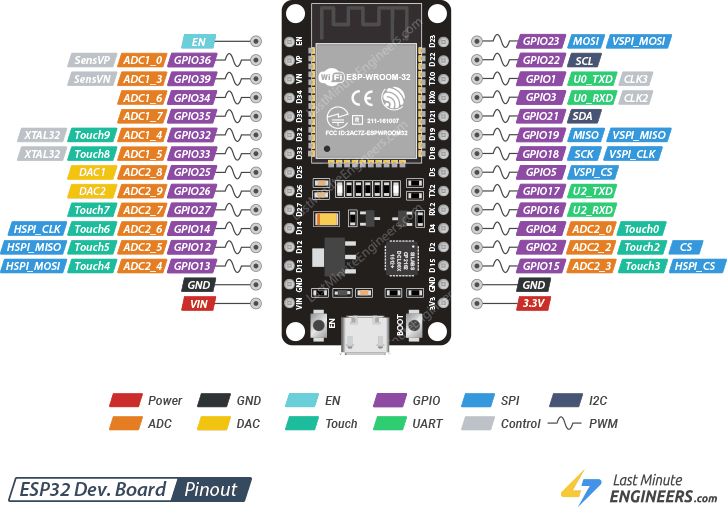
\includegraphics[width=0.8\textwidth]{Images/WP1_2/Tache_0/ESP32.png}
    \caption{Pinout Diagramme de l'ESP32}
\end{figure}

\noindent\textit{Notes :}  
Un document détaillé présentant l’analyse comparative entre l’ESP32 et le Raspberry Pi Zero, ainsi que les critères de sélection, 
à été rédigé.

\subsubsection{Tache 1 : Gestion du stockage des données collectées}

\subsubsection*{Rappel des objectifs}

Commençons par la tache 1 qui est la gestion du stockage des données collectées. Pour cette tache, il a été décidé d'utiliser 
une carte SD ( par cahier des charges ) pour stocker les données collectées par les métadatas et images. La carte SD offre une grande 
capacité de stockage, ce qui est essentiel pour notre projet De plus, les cartes SD sont relativement faciles à interfacer avec un 
microcontrôleur, ce qui facilite l'intégration dans notre système. Enfin celle ci est facilement accessible pour les utilisateurs, 
ce qui permet une récupération facile des données collectées.
\\

Dons nous avons utilisé un module de carte SD utilisable en moyen de communication SPI, qui est un protocole de communication série rapide 
et efficace. Le microcontrôleur peut ainsi envoyer des commandes à la carte SD pour lire et écrire des données de manière rapide et fiable.
Le module utilisé est un module personnel ( \texttt{AZDelivery SPI Reader} ), celui-ci à été choisi au début du projet car aucune
commande n'étais envisageable de la part du département ou du client.
\\

\begin{figure}[H]
    \centering
    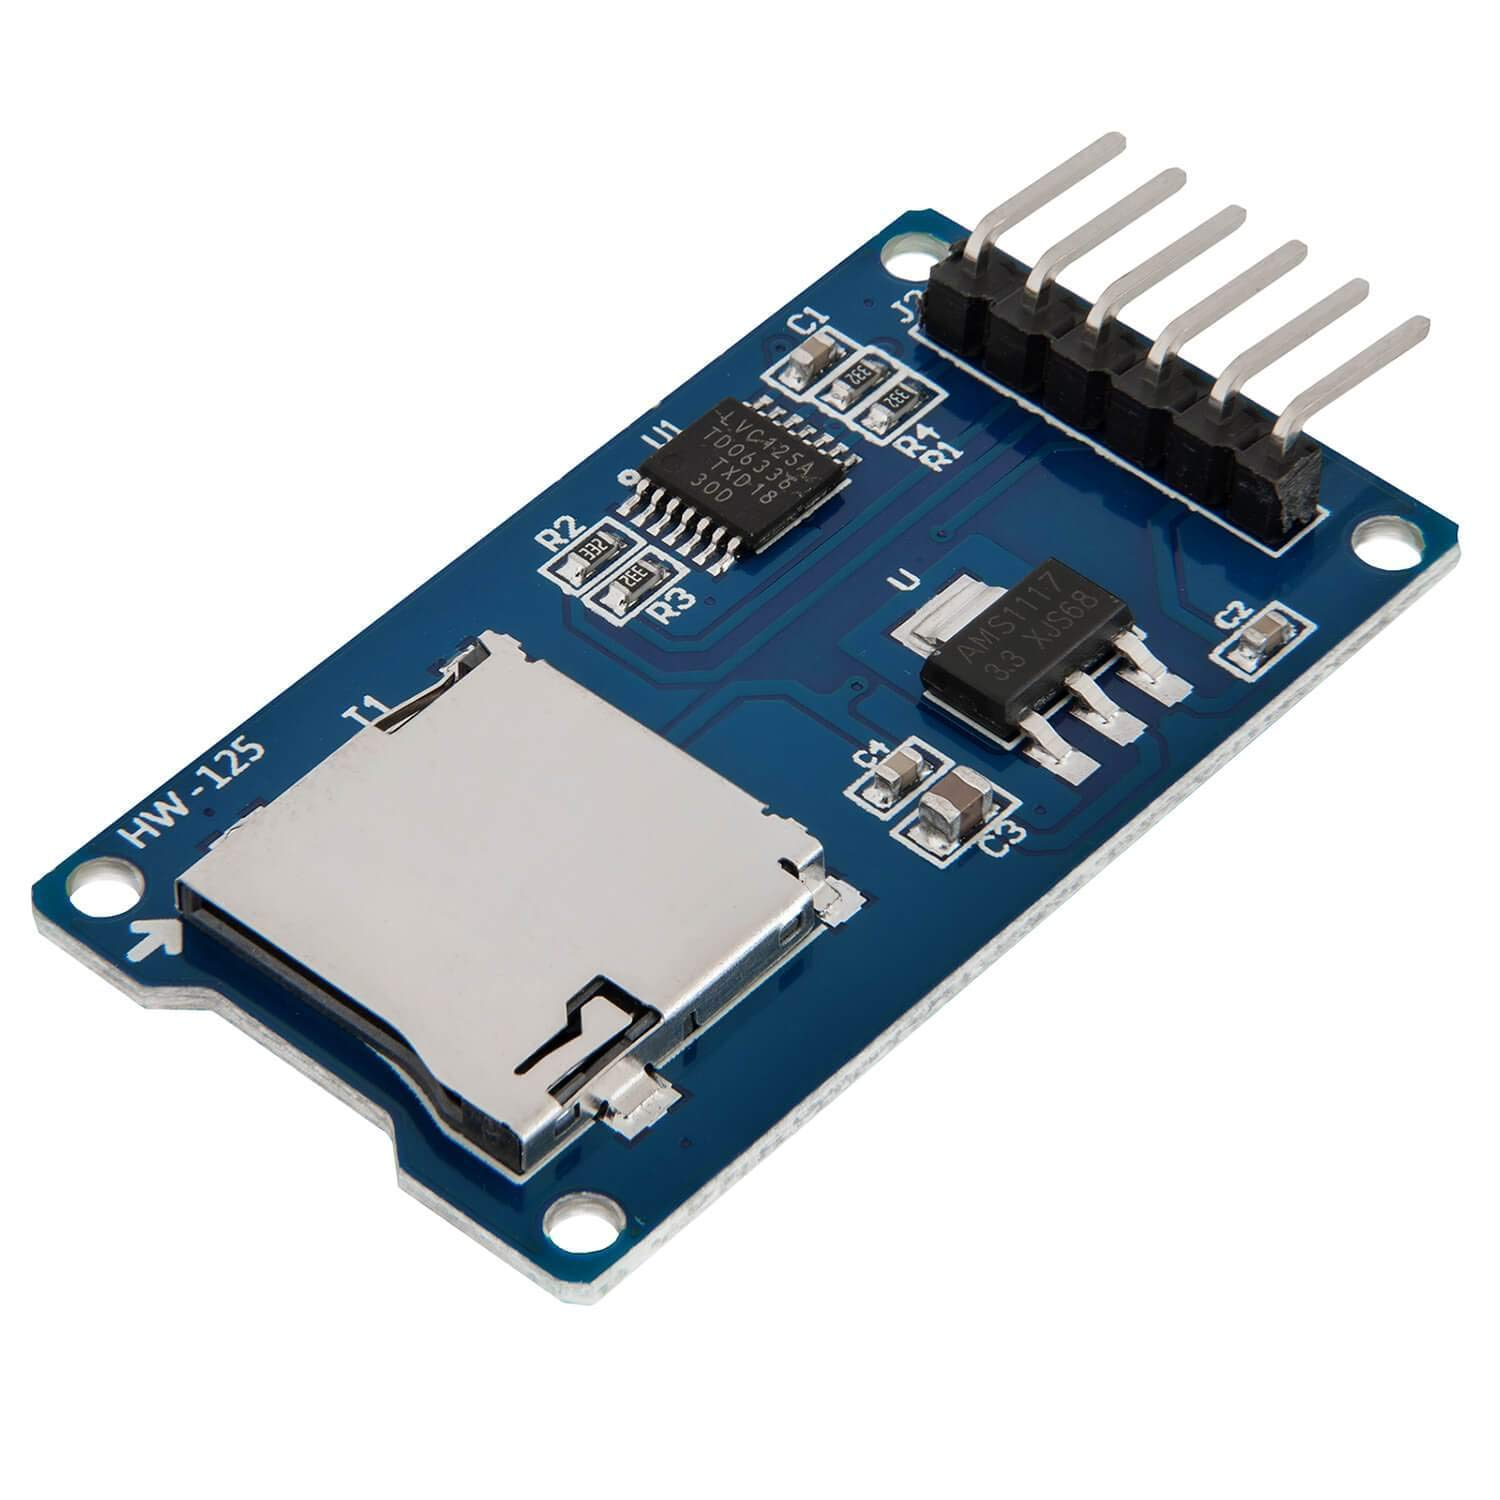
\includegraphics[width=0.4\textwidth]{Images/WP1_2/Tache_1/ModuleSD.jpg}
    \caption{Module de carte SD utilisé pour le projet}
\end{figure}

\subsubsection*{Solution envisagée}

Pour utilisé le module, nous avons connecté notre esp32 à ce module en liaison SPI, en utilisant les broches suivantes :
\begin{itemize}
    \item MOSI ( Master Out Slave In : Écriture ) : GPIO 13
    \item MISO ( Master In Slave Out : Lecture ) : GPIO 12
    \item SCK ( Serial Clock ) : GPIO 14
    \item CS ( Chip Select ) : GPIO 15
    \item VCC : 5V
    \item GND : GND
    \\
\end{itemize}

Nous utiliserons le module HSPI de l'ESP32 pour la communication SPI, qui permet des vitesses de transfert élevées.
Voici un exmple de communication en SPI pour décrire le moyen de communication entre l'ESP32 et la carte SD. 

\begin{figure}[H]
    \centering
    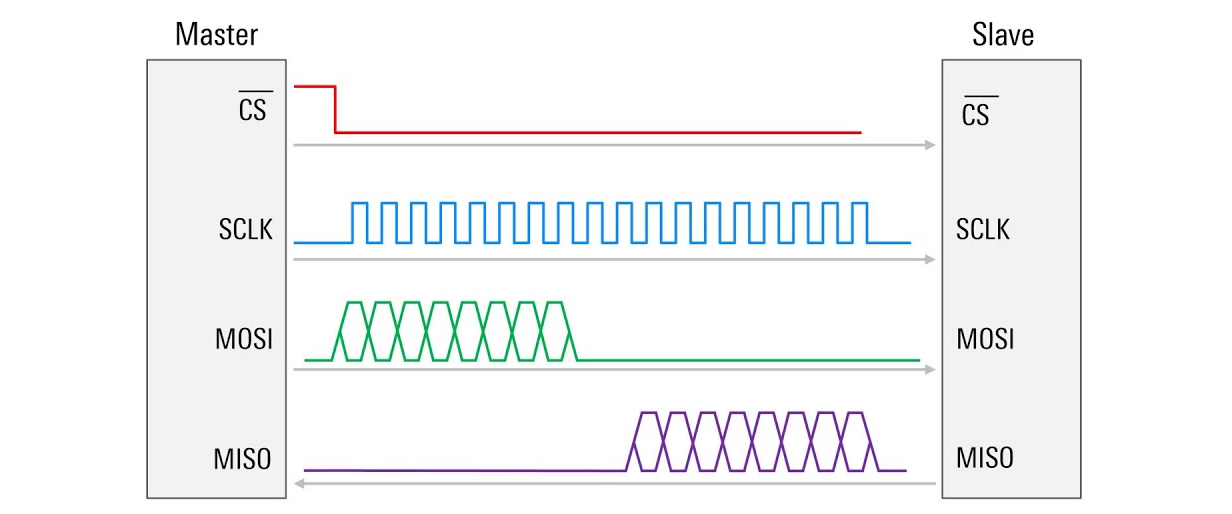
\includegraphics[width=0.8\textwidth]{Images/WP1_2/Tache_1/SPI.png}
    \caption{Module de carte SD utilisé pour le projet}
\end{figure}


Pour utiliser ce module, une librairie toute faite à déja été développé, qu'il à suffit d'implémenter dans notre projet pour pouvoir 
utilisé la carte SD. Cette librairie est la librairie \texttt{SD.h} qui est une librairie standard pour la gestion des cartes SD avec 
les microcontrôleurs Arduino et ESP32. Elle offre des fonctions pour initialiser la carte SD, lire et écrire des fichiers, 
et gérer les répertoires. Nous l'avons utilisé pour crée ntre propre bibliothèque visant à simplificer l'utilisation de cette carte avec 
notement le WPBis qui est dédier à la gestion de la transmission des données collectées.
\\

\subsubsection*{Tests et Validation}

Pour la phase de test, nous avons juste réalisé un test afin de savoir si nous pouvions écrire un fichier texte sur la carte SD,
En donnant comme Nom de fichier les métadatas ( comme température, humidité, etc ), afin de simulé un buffer de réception d'images avec 
les données correspondantes.
\\

Voici un exemple de code utilisé pour ce test :

\begin{lstlisting}[style=CStyle, caption={Exemple utilisation module SD}, label={lst:sd_exemple}]
#include <SD_PIEGE.h>

void setup()
{ 
    initSD(); 
    
    // Temperature_Humidite_Latitude_Longitude_Heure_Minute_Seconde
    String filename = "20_60_47-2833012_1-5152623_10-30-30.txt"; 
    
    File file = SD.open(filename, FILE_WRITE); 
    
    // Exemple de donnees JPEG 
    uint8_t image[] = {0xFF, 0xD8, 0xFF, 0xE0, 0x00, 0x10, 0x4A, 0x46}; 
    
    file.write(image, sizeof(image)); 
    file.close(); 
}
\end{lstlisting}

\begin{figure}[H]
    \centering
    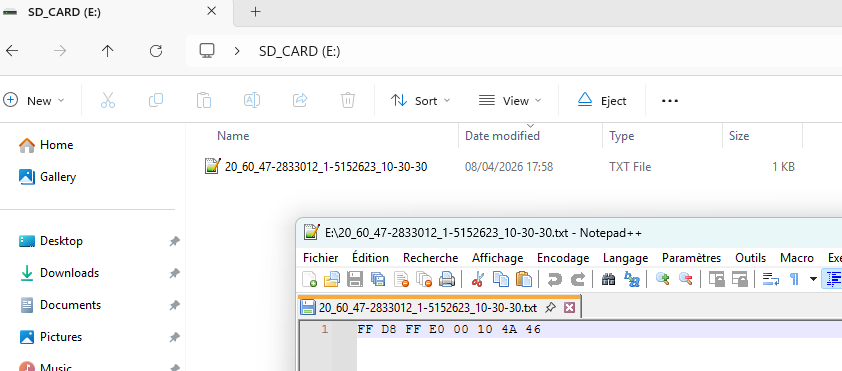
\includegraphics[width=0.8\textwidth]{Images/WP1_2/Tache_1/Result_SD.png}
    \caption{Résultat du test d'écriture sur la carte SD}
\end{figure}

\subsubsection{Tache 2 : Hors WP : Gestion de la luminosité pour WP 1.3}

\subsubsection*{Rappel des objectifs}

Pour cette partie nous avons décidé de me séparé de mon WP afin d'aider le 
WP 1.3 qui est dédié à la gestion de la caméra, notamment pour la partie de 
la luminosité. En effet, la luminosité est un facteur important pour la 
prise de vue des images, car d'après notre cahier des charges, nous voulions
prendre des photographie de jour comme de nuit. 
\\

Avoir la possibilité de connaitre la luminosité de l'environnement, nous permettrai
de pourvoir allumer une source de lumière ( comme des LED Infrarouge ) pour pouvoir
capturer des élement de nuit.
\\

\subsubsection*{Solution envisagée}

Pour cela nous avons décidé d'ajouter un capteur de luminosité ( une photorésistance ( LDR )) 
afin de capturer la luminosité de l'environnement. Ce capteur est un composant électronique 
qui change de résistance en fonction de la quantité de lumière. C'est un capteur très simple à mettre
en œuvre et à interfacer avec un microcontrôleur comme l'ESP32. En mesurant la résistance de la 
photorésistance, nous pouvons déterminer la luminosité ambiante et ajuster le comportement de notre système.
\\

Pour connaitre la résistance de ce capteur, nous utilisons un montage de diviseur de tension, 
qui nous permet de convertir la résistance variable de la photorésistance en une tension mesurable par l'ESP32.
Voici un schéma de ce montage :
\\

%\begin{figure}[H]
%    \centering
%    \includegraphics[width=0.8\textwidth]{Images/WP1_2/Tache_2/Diviseur_Tension.png}
%    \caption{Schéma du montage de diviseur de tension pour la photorésistance}
%\end{figure}

Dans ce montage, la photorésistance ( LDR ) est connectée en série avec une résistance fixe ( R1 ).
Lorsque la lumière frappe la photorésistance, sa résistance change, ce qui modifie la tension de sortie ( Vout ) du diviseur de tension.
En mesurant cette tension de sortie avec l'ESP32, nous pouvons calculer la résistance de la photorésistance et ainsi déterminer la luminosité ambiante.
\\

\[
    R_{LDR} = (( R_{serie} * 3.3 ) / Tension_{Vout} ) - R_{serie};
\]


A partir de la documention technique de la LDR nous pouvons facilement retrouver la valeur
de la luminausité ( en LUX ) à partir de la résistance de la résistance, en utilisant la courbe suivante :
\\

\begin{figure}[H]
    \centering
    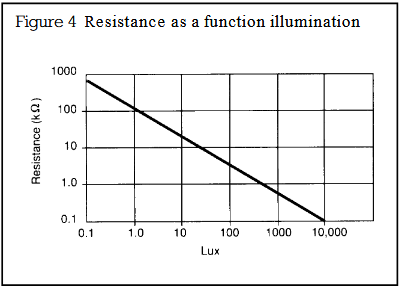
\includegraphics[width=0.8\textwidth]{Images/WP1_2/Tache_2/CourbeLDR.png}
    \caption{Courbe de résistance en fonction de la luminosité pour la photorésistance}
\end{figure}

\[
    Lux = (\frac{1000}{Resistance})^{1.4}   
\]

\subsubsection*{Tests et Validation}

Pour la phase de test de cette LDR nous avons tous simplement effectué 
plusieur mesure avec des taux de luminosité différent, en utilisant une lampe, chiffon, rideau, etc ... 
pour faire varier la luminosité, et en mesurant la tension de sortie du diviseur de tension.
\\

Pour lire la valeur numérique nous avons tout simplement utilisé la fonction \texttt{analogRead()} de l'ESP32, 
qui nous permet de lire la tension de sortie.
\\

Voici un exemple de code utilisé pour ce test :

\begin{lstlisting}[style=CStyle, caption={Exemple utilisation LDR}, label={lst:ldr_exemple}]
#define LDR_PIN 34 // Broche analogique pour la LDR
#define RESISTOR_BRIDGE 10000 // Resistance diviseur de tension 

void setup() 
{
    Serial.begin(115200); 
}

void loop() 
{
    // Calcul de la tension ( ADC 12 bits )
    ldrValue = (analogRead(LDR_PIN) * 3.3) / (1.0 * 4095.0);

    // Calcul de la reistance 
    float resistance = (( RESISTOR_BRIDGE * 3.3 ) / ldrValue ) - RESISTOR_BRIDGE;
    
    // Calcul de la luminosite en LUX
    float lux = pow((1000 / resistance), 1.4); 

    Serial.print("LDR Value: ");
    Serial.println(ldrValue); // Affichage de la valeur lue
    
    Serial.print("Resistance: ");
    Serial.println(resistance); // Affichage de la resistance calculee
    
    Serial.print("Luminosite (LUX): ");
    Serial.println(lux); // Affichage de la luminosite calculee

    delay(1000); // Attente d'une seconde avant la prochaine lecture
}
\end{lstlisting}

Avec ce code nous avons pu vérifier que notre capteur LDR fonctionnait comme un luxmètre,
en affichant la valeur de luminosité en LUX dans le moniteur série de l'ESP32. 
Nous avons en même temps vérifier à l'aide d'une lumètre ( téléphone ) que les valeurs de 
luminosité affichées étaient cohérentes avec les mesures réelles. Malheureusement le téléphone 
utilisant une application celui-ci n'était pas très précis.
\\

Mais dans l'ensemble des résultats obtenus étaient cohérents, on a obtenue : 
\\

\begin{table}[H]
    \centering
    \footnotesize
    \setlength{\tabcolsep}{3pt}
    \renewcommand{\arraystretch}{1.15}
    \resizebox{\textwidth}{!}{%
    \begin{tabular}{|l|c|c|c|c|c|c|c|c|c|}
        \hline
        & \multicolumn{3}{c|}{\textbf{Theorie (Calcul)}} & \multicolumn{3}{c|}{\textbf{Numerique (Code)}} & \multicolumn{3}{c|}{\textbf{Pratique (Multimetre + Tel)}} \\
        \cline{2-10}
        & \textbf{Tension} & \textbf{Resistance} & \textbf{Lux} & \textbf{Tension} & \textbf{Resistance} & \textbf{Lux} & \textbf{Tension} & \textbf{Resistance} & \textbf{Lux (PAS FIABLE)} \\
        \hline
        \textbf{Noir (Torchon)} & 0 & 1M & 0,1 & 0 & 1M & 1 & 0 & 17,16M & 0 \\
        \hline
        \textbf{Sombre} &  &  &  & 0,69 & 5668 & 2636 & 0,7 & 5300 & 100 \\
        \hline
        \textbf{Gris} &  &  &  & 2 & 996 & 10000 & 2,13 & 890 & 500 \\
        \hline
        \textbf{Lumiere} &  &  &  & 2,71 & 329 & 10000 & 2,8 & 237 & 1900 \\
        \hline
        \textbf{Flash} & 3,3 & 0,1 & 10000 & 3,3 & 0 & 10000 & 3,22 & 72,3 &  \\
        \hline
    \end{tabular}
    }
    \caption{Comparaison des mesures de luminosite : theorie, calcul numerique et mesures pratiques}
    \label{tab:ldr_comparaison}
\end{table}

\subsubsection{Tache 3 : Gestion de l'horodatage et de la localisation du modules}

\subsubsection*{Rappel des objectifs}

Pour cette tache, nous avons décidé d'ajouter un module GPS afin de pouvoir récupérer la localisation du module, ainsi que l'heure 
grâce à ce module. En effet, les données d'horodatage sont necessaires pour pouvoir avoir des statistique sur le taux
de passage dans la zone en question, et la localisation est nécessaire dans le cas nous aurions plusieurs modules à déployer, afin 
d'observer les zonnes de passage.
\\

Nous avons décidé d'utiliser un module GPS personnel ( dans le même cas que pour la carte SD, aucune commande n'était envisageable de 
la part du département ou du client ), qui est un module basique déstiné plutot pour les drones FPV.
\\

\begin{figure}[H]
    \centering
    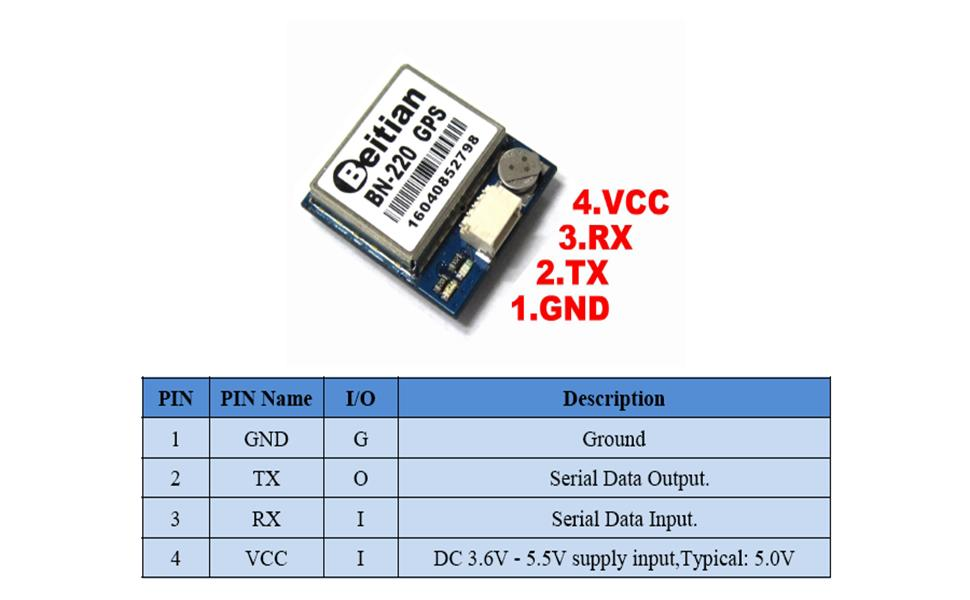
\includegraphics[width=0.8\textwidth]{Images/WP1_2/Tache_3/BN220.jpg}
    \caption{Module GPS utilisé pour le projet}
\end{figure}

\subsubsection*{Solution envisagée - GPS}

Ce module est basé sur une communication Série UART, qui est un protocole de communication simple et largement utilisé pour les modules GPS.
Celui ci envoie des données de localisation et d'horodatage au format NMEA, qui est un format standard pour les données GPS.
Différentes trames NMEA contiennent différentes informations, telles que la position, la vitesse, l'heure, etc. 
\\

Pour exemple la trame la plus connue est celle de GGA, qui est : 
\\

\begin{figure}[H]
    \centering
    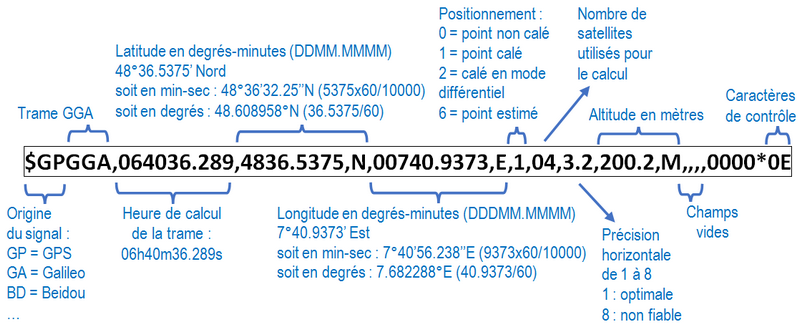
\includegraphics[width=0.8\textwidth]{Images/WP1_2/Tache_3/tramenmea.png}
    \caption{Exemple de trame NMEA envoyée par le module GPS}
\end{figure}

Dans notre cas nous allons utiliser la trame \texttt{GPRMC} :

\begin{figure}[H]
    \centering
    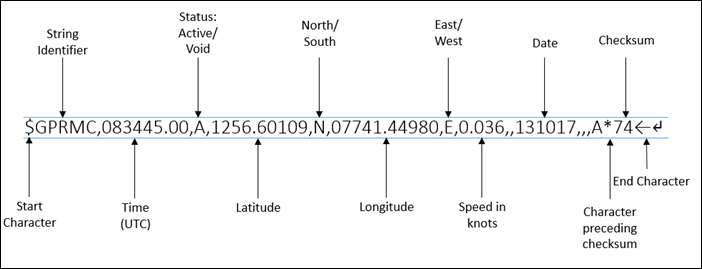
\includegraphics[width=0.8\textwidth]{Images/WP1_2/Tache_3/GPRMC.png}
    \caption{Trame GPRMC utilisée pour récupérer la localisation et l'horodatage}
\end{figure}

Grace à cette trame, nous allons pouvoir récupérer l'heure ( UTC ), la latitude, la longitude.
\\

Pour l'implémentation de ce module, nous avons crée notre librairie Arduino visant à récuper les informations que 
nous shouaitons à partir des information communication en liaisons UART. 
\\

Le principe est simple nous attendons qu'une trame complète soit arrivée, nous anaylison sur le carractère du début est bien \texttt{\$GPRMC} 
et nous analysons les caractère qui sont séparé par des virgules pour récupérer les différentes informations.
A la suite de ça nous avons crée une class en c permettant de pouvoir récupér les valeur directement via une simple fonction, \texttt{get()}.
\\

\subsubsection*{Solution envisagée - RTC}

Pour la partie du GPS nous avons pu voir que nous pouvions récupérer toute les inforamtions néecssaire à notre projet,
cependant il y avait un probleme, le GPS met du temps à se capter la localisation car celui-ci dépend de la position des 
satellites, et dans le cas ou le module est dans une zone isolé, il peut mettre du temps à se capter la localisation.
\\

Une solution était d'utiliser un module RTC ( Real Time Clock ), celui si permettrait de continuer à obtenir l'heure sans pour autant
avoir besoin d'utiliser le module GPS, ce qui nous permettrait de gagner du temps sur tout le cheminement de la capture à la transmission.
\\

Un module RTC est un composant électronique qui maintient une horloge en temps réel, même lorsque le microcontrôleur est éteint ou redémarré.
Voici un schéma du principe que nous voulions implémenter : 
\\

\begin{figure}[H]
    \centering
    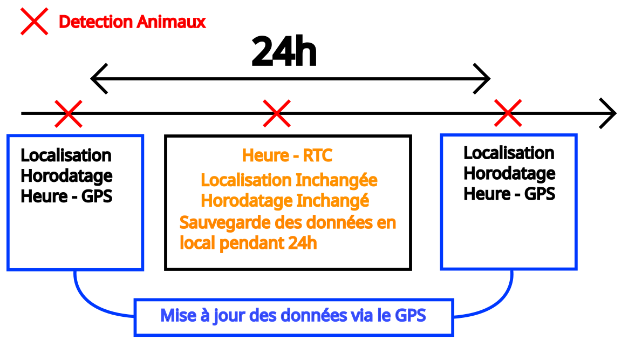
\includegraphics[width=0.8\textwidth]{Images/WP1_2/Tache_3/Schema_GPS.png}
    \caption{Schéma du principe de fonctionnement du module RTC pour maintenir l'heure en temps réel}
\end{figure}

Pour l'implémentation de ce module, nous avons implémenter notre propre librairie qui vise à récupérer 




\subsubsection*{Tests et Validation}

